% !TEX root = MAIN.tex

\clearpage

\section{GSL - libgcsp}
\label{sec:caseStudies:GSL:libgcsp}

\subsection{Overview of the case study}

The GomSpace CSP library (libgscsp) is a GomSpace extension to the open source CubeSat Space Protocol library.
The GomSpace CSP library provides:
\begin{itemize}
\item convenience wrapping of CSP functionality, primarily initialization.
\item definition of standard CSP ports (used by other GomSpace products).
\item connecting low-level drivers (e.g. CAN, I2C from Embed library) with CSP interfaces 
\item generic CSP service dispatcher, forwards incoming connections to service handlers.
\end{itemize}

The libgscsp contains a GomSpace branch (https://github.com/GomSpace/libcsp) of the open source libcsp (https://github.com/libcsp/libcsp), located in the subfolder lib/libcsp. The two libcsp branches are kept as identical as possible, as features specific to GomSpace are placed in libgscsp.

Details about libgscsp are provided in the document \emph{gs-man-nanosoft-ms100-command-and-management-sdk-3.6.2-1-g67fe6e1.pdf} uploaded on Alfresco.


The size of libgscsp is 1\,497 LOC, %include 306, src 1776+15 = total = 1497
while libcsp (GSL branch) is 8\,339 LOC. % 6789 + 1550
Instead, the libgscsp unit test suite consists of 89 test cases, compiled and executed through the WAF meta-build system.

\subsection{Code-driven mutation testing}

\DONE{Can we provide separate information about the code coverage for libgscsp (no libcsp branch) and for libcsp branch?}

\DONE{Clarify which components we mutate}

We have seen that a mutant can be killed only if it is covered by at least one test case. For this reason, the code-driven mutation testing process in libgscsp will target all the components covered by the libgscsp unit test suite.

% !TEX root = ../MAIN.tex

\begin{table}[h]

\footnotesize
\parbox{.45\linewidth}{
\centering
\begin{tabular}{|l|l|}
\hline
\textbf{Coverage Type} & \textbf{Coverage Rate} \\
\hline
Statement     & 58.4\% (390 of 668 statements)\\
Functions     & 71.4\% (50 of 70 functions)\\
Branches      & 41.2\% (165 of 400 branches)\\
\hline
\end{tabular}
\caption{libgscsp code coverage.}
\label{table:libgscsp_coverage}
}
\hfill
\parbox{.45\linewidth}{
\centering
\begin{tabular}{|l|l|}
\hline
\textbf{Coverage Type} & \textbf{Coverage Rate} \\
\hline
Statement     & 64.1\% (2112 of 3297 statements)\\
Functions     & 72.5\% (248 of 342 functions)\\
Branches      & 44.9\% (989 of 2201 branches)\\
\hline
\end{tabular}
\caption{libcsp code coverage.}
\label{table:libcsp_coverage}
}
\end{table}	

\begin{enumerate}
	\item \textbf{libgscsp}

	Table~\ref{table:libgscsp_coverage} provides code coverage information of the libgscsp unit test suite for the GSL extension to the CSP library. Given the code coverage, we focus our analysis to the following subset of components (i.e., components with code coverage greater than 0\%):

	\begin{itemize}
	 	\item src/clock.c
	 	\item src/commands.c
	 	\item src/conn.c
	 	\item src/csp.c
	 	\item src/error.c
	 	\item src/log.c
	 	\item src/router.c
	 	\item src/service\_dispatcher.c
	 	\item src/service\_handler.c
	 	\item src/linux/command\_line.c

	 \end{itemize} 

	\item \textbf{libcsp (GSL branch)}

	Table~\ref{table:libcsp_coverage} presents the code coverage of the libgscsp unit test suite for the GSL branch of the CSP library.  Given the code coverage, we focus our mutation analysis on the following subset of components (i.e., components with code coverage greater than 0\%):

	\begin{itemize}
		\item src/arch/csp\_time.c
		\item src/arch/csp\_system.c
		\item src/arch/posix/csp\_thread.c
		\item src/arch/posix/csp\_semaphore.c
		\item src/arch/posix/csp\_malloc.c
		\item src/arch/posix/csp\_queue.c
		\item src/arch/posix/csp\_time.c
		\item src/arch/posix/pthread\_queue.c
		\item src/arch/posix/csp\_system.c
		\item src/crypto/csp\_sha1.c
		\item src/crypto/csp\_hmac.c
		\item src/crypto/csp\_xtea.c
		\item src/interfaces/csp\_if\_lo.c
		\item src/rtable/csp\_rtable.c
		\item src/rtable/csp\_rtable\_cidr.c
		\item src/rtable/csp\_rtable\_static.c
		\item src/transport/csp\_rdp.c
		\item src/transport/csp\_udp.c
		\item src/csp\_sfp.c
		\item src/csp\_debug.c
		\item src/csp\_service\_handler.c
		\item src/csp\_crc32.c
		\item src/csp\_io.c
		\item src/csp\_qfifo.c
		\item src/csp\_iflist.c
		\item src/csp\_endian.c
		\item src/csp\_route.c
		\item src/csp\_buffer.c
		\item src/csp\_port.c
		\item src/csp\_conn.c
		\item src/csp\_init.c
		\item src/csp\_services.c
	\end{itemize}


\end{enumerate}

\subsubsection{Mutation Testing Preliminary Results}

\DONE{We can add some preliminary results}

% !TEX root = ../MAIN.tex

\begin{table}[h]
\small
\centering
\caption{Code-driven mutation testing preliminary results for the libgscsp case study.}
\label{table:libgscsp_preliminary}
\begin{tabular}{|l|l|l|l|l|l|l|}
\hline
        & \multicolumn{5}{c|}{Mutants}                                                                      & \multirow{3}{*}{\begin{tabular}[c]{@{}l@{}}Mutation Score\\ (K/K+L)\end{tabular}} \\ \cline{1-6}
        &     &                                                        &      & \multicolumn{2}{c|}{Killed} &                                                                                   \\ \cline{1-6}
Mutants & All & \begin{tabular}[c]{@{}l@{}}Not\\ Compiled\end{tabular} & Live & Test Failure    & Timeout   &                                                                                   \\ \hline
Total   &  6\,196   &  1\,700 & 1\,708      & 2\,495                & 277          & 61.88\%                                                                           \\ \hline
\end{tabular}
\end{table}    
             

In order to analyze the feasibility of the code-driven mutation testing for libgscsp, we conducted a preliminary experimentation using the mutation operators AOR, ROR, ICR, LCR, ABS, UOI and SDL we generated 6\,196 mutants. For the experimentation we consider only the libcsp (GSL branch) source code. Preliminary results can be found in Table~\ref{table:libgscsp_preliminary}.
Particularly, we observe that from the 6\,196 generated mutants, we had 1\,700 mutants that were not compiled by the compilation toolset of libgscsp, most probably because the mutation introduced a syntactical error that was detected by the toolset.
Then, we identified 1\,708 live mutants that were not detected by the test suite. Instead, we had 2\,495 killed mutants detected by the test suite, and 277 mutants that produced libutil to go into an infinite loop, and thus were killed by timeout. The final mutation score was of 61.88\%.

The identification of equivalent mutants still needs to be assessed.


\subsection{Data-driven mutation testing}

\DONE{We should indicate the functions we mutate.}

The data-driven mutation testing process in libgscsp will target the data packet transferred between the server and the client using the CSP protocol. Specifically, the mutations will affect the header of the packet, in general the routing information (see Figure~\ref{fig:csp_packet}), and the payload of the packet.

\begin{figure}[h]
  \centering
    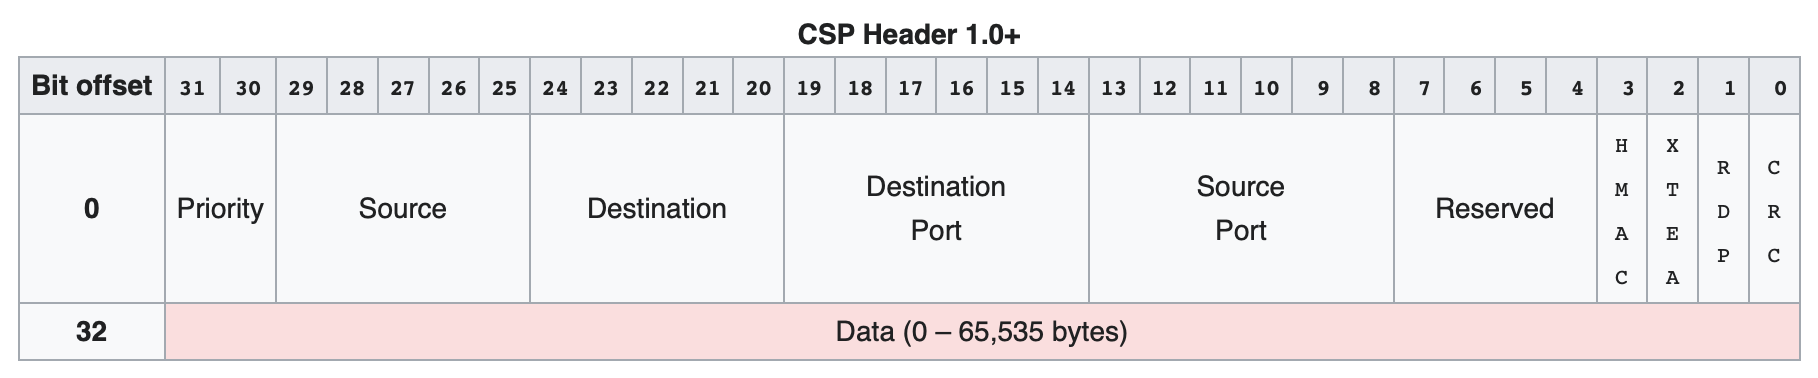
\includegraphics[width=0.9\textwidth]{images/csp_packet}
      \caption{CSP protocol header.}
      \label{fig:csp_packet}
\end{figure}


% !TEX root =  ../MAIN.tex

\begin{minipage}{16cm}
\begin{lstlisting}[style=CStyle, caption=Data-driven mutation example on libgscsp (csp\_io.c excerpt)., label=csp_integration]
unsigned int v[6] = {packet->id.flags, packet->id.sport, packet->id.dport, 
                    packet->id.dst, packet->id.src, packet->id.pri};

FaultModel *fm = _FAQAS_Identifier_FM();                                                                                          
mutate(v, fm);
_FAQAS_delete_FM(fm);

packet->id.flags = v[0];
packet->id.sport = v[1];
packet->id.dport = v[2]; 
packet->id.dst = v[3]; 
packet->id.src = v[4]; 
packet->id.pri = v[5]; 
\end{lstlisting}
\end{minipage}


Both mutations (i.e, header and payload) will be performed before the message is serialized. 
For example, the mutations to the header will affect the csp\_send\_direct function of the csp\_io component. Listing~\ref{csp_integration} shows an example of our data-driven mutator prototype within the csp\_io component. Particularly, the packet header is translated into an unsigned int vector, which is then passed to the FAQAS mutate function, here a fault model could be applied to all six items of the header. After the mutation is applied the vector is translated back again to the original representation.
 

\section{GSL - libparam}
\label{sec:caseStudies:GSL:libparam}

\subsection{Overview of the case study}

The Parameter System (i.e., libparam) is a light-weight parameter system designed for GomSpace satellite subsystems. It is based around a logical memory architecture, where every parameter is referenced directly by its logical address. A backend system takes care of translating addresses into physical addresses.
The features of this system include:
\begin{itemize}
\item Direct memory access for quick parameter reads.
\item Simple data types: uint, int, float, double, string.
\item Arrays of simple data types.
\item Supports multiple stores per table, e.g. FRAM, MCU flash, file (binary or text).
\item Remote client with support for most features (rparam).
\item Packed GET, SET queries, supporting multiple parameter set/get in a single request. Data serialization and deserialization.
\item Supports both little and big-endian systems.
\item Commands for both local (param) and remote access (rparam).
\item Parameter server for remote access over CSP.
\item Compile-time configuration of parameter system
\end{itemize}

Details about libparam are provided in the document \emph{gs-man-nanosoft-ms100-command-and-management-sdk-3.6.2-1-g67fe6e1.pdf} uploaded on Alfresco.

\subsection{Code-driven mutation testing}

\TODO{We do it or not?}

\subsection{Data-driven mutation testing}

\TODO{We should indicate the functions we mutate}


\section{GSL - libutil}
\label{sec:caseStudies:GSL:libutil}

\subsection{Overview of the case study}

The Utility library provides cross-platform APIs for common functionality, for use in both embedded systems and standard PCs running Linux. 

Details about libutil are provided in the document \emph{gs-man-nanosoft-ms100-command-and-management-sdk-3.6.2-1-g67fe6e1.pdf} uploaded on Alfresco.

The size of libutil is 10\,576 LOC, while the unit test suite consists of 201 test cases written in C.

\subsection{Code-driven mutation testing}

\DONE{Add some details about what we mutated}

The code-driven mutation testing process in libutil will target all the components covered by the libutil unit test suite. 

% !TEX root = ../MAIN.tex

\begin{table}[h]

\centering
\begin{tabular}{|l|l|}
\hline
\textbf{Coverage Type} & \textbf{Coverage Rate} \\
\hline
Statement     & 83.2\% (8\,817 of 10\,596 statements)\\
Functions     & 82.1\% (725 of 883 functions)\\
Branches      & 56.6\% (2\,618 of 4\,627 branches)\\
\hline
\end{tabular}
\caption{libutil code coverage.}
\label{table:gslibutil_coverage}

\end{table}

Table~\ref{table:gslibutil_coverage} provides the code coverage information of the unit test suite for the GSL libutil library. Given the code coverage, we focus our analysis to the following subset of components (i.e., components with code coverage greater than 0\%):

\begin{itemize}
	\item src/base16.c
	\item src/bytebuffer.c
	\item src/byteorder.c
	\item src/clock.c
	\item src/crc32.c
	\item src/crc8.c
	\item src/error.c
	\item src/fletcher.c
	\item src/function\_scheduler.c
	\item src/hexdump.c
	\item src/lock.c
	\item src/rtc.c
	\item src/string.c
	\item src/strtoint.c
	\item src/time.c
	\item src/timestamp.c
	\item src/cmd/command.c
	\item src/cmd/log.c
	\item src/cmd/vmem.c
	\item src/drivers/sys/memory.c
	\item src/gosh/command.c
	\item src/gosh/console.c
	\item src/gosh/default\_commands.c
	\item src/linux/clock.c
	\item src/linux/command\_line.c
	\item src/linux/cwd.c
	\item src/linux/delay.c
	\item src/linux/function.c
	\item src/linux/mutex.c
	\item src/linux/queue.c
	\item src/linux/rtc.c
	\item src/linux/sem.c
	\item src/linux/signal.c
	\item src/linux/stdio.c
	\item src/linux/thread.c
	\item src/linux/time.c
	\item src/linux/drivers/gpio/gpio.c
	\item src/linux/drivers/gpio/gpio\_sysfs.c
	\item src/linux/drivers/gpio/gpio\_virtual.c
	\item src/linux/drivers/i2c/i2c.c
	\item src/linux/drivers/spi/spi.c
	\item src/linux/drivers/sys/memory.c
	\item src/log/commands.c
	\item src/log/log.c
	\item src/log/appender/console.c
	\item src/log/appender/simple\_file.c
	\item src/test/cmocka.c
	\item src/test/command.c
	\item src/test/log.c
	\item src/vmem/commands.c
	\item src/vmem/vmem.c
	\item src/watchdog/monitor\_task.c
	\item src/watchdog/watchdog.c
	\item src/zip/zip.c
	\item src/zip/miniz/miniz.c
\end{itemize}

\subsubsection{Mutation Testing Preliminary Results}

\DONE{We can add some preliminary results}

% !TEX root = ../MAIN.tex

\begin{table}[h]
\small
\centering
\caption{Code-driven mutation testing preliminary results for the libutil case study.}
\label{table:libutil_preliminary}
\begin{tabular}{|l|l|l|l|l|l|l|}
\hline
        & \multicolumn{5}{c|}{Mutants}                                                                      & \multirow{3}{*}{\begin{tabular}[c]{@{}l@{}}Mutation Score\\ (K/K+L)\end{tabular}} \\ \cline{1-6}
        &     &                                                        &      & \multicolumn{2}{c|}{Killed} &                                                                                   \\ \cline{1-6}
Mutants & All & \begin{tabular}[c]{@{}l@{}}Not\\ Compiled\end{tabular} & Live & Test Failure    & Timeout   &                                                                                   \\ \hline
Total   &  16\,886   &  2\,561                                                      & 3\,402      & 10\,634                & 289          & 76.25\%                                                                           \\ \hline
\end{tabular}
\end{table}    
             

In order to analyze the feasibility of the code-driven mutation testing, we conducted a preliminary experimentation using the mutation operators AOR, ROR, ICR, LCR, and SDL we generated 16\,886 mutants. Preliminary results can be found in Table~\ref{table:libutil_preliminary}.
Particularly, we observe that from the 16\,886 generated mutants, we had 2\,561 mutants that were not compiled by the compilation toolset of libutil, most probably because the mutation introduced a syntactical error that was detected by the toolset.
Then, we identified 3\,402 live mutants that were not detected by the test suite. Instead, we had 10\,634 killed mutants detected by the test suite, and 289 mutants that produced libutil to go into an infinite loop, and thus were killed by timeout. The final mutation score was of 76.25\%.

The identification of equivalent mutants still needs to be assessed.


\subsection{Data-driven mutation testing}

We do not plan to apply data drive mutation testing to this case study because is a standalone library; it does not integrate communicating components.
